\section{Causality}

\begin{frame}{Causality}
    \begin{itemize}
        \item Halpern and Pearl developed mathematical formulation of causality
        \item It involves counterfactuals, statements counter to fact
        \item Event A is said to be a cause of event B if, had A not happened then B would not have happened
        \item It does not consider just what actually happened but also what might have happened, had things been different
    \end{itemize}
\end{frame}

\begin{frame}{Causality: Counterfactuals}
    \begin{figure}
        \centering
        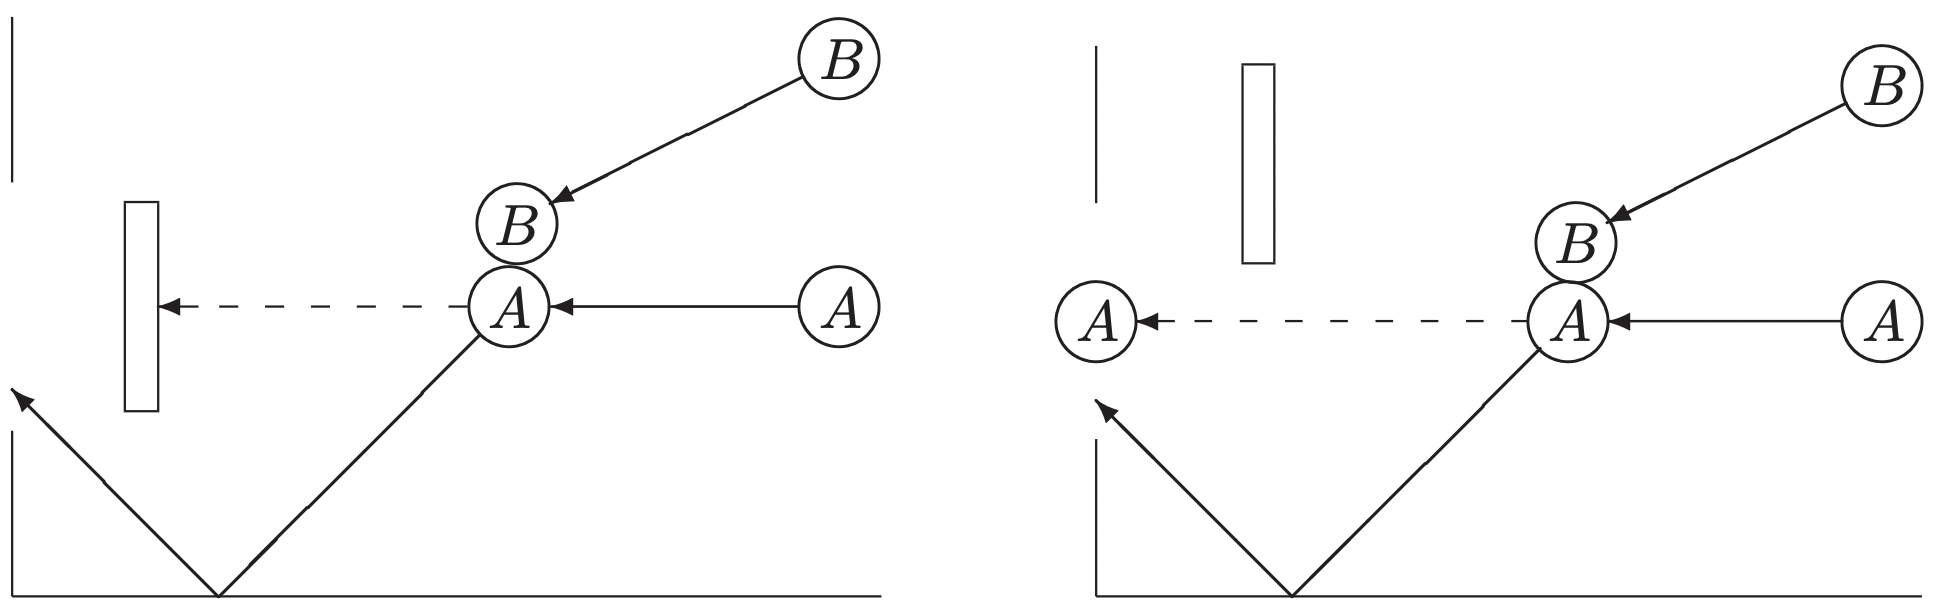
\includegraphics[width=10cm]{resources/balls.png}
    \end{figure}
    \begin{itemize}
        \item $A$ going toward the goal, $B$ hits $A$
        \item $A$ banks of the wall and goes into the goal
        \item Two scenarios, a brick blocks the A's path in the left scenario
        \item Is $B$ hitting the ball caused $A$ to go into the goal?
        \item The dashed path is a result of a counterfactual
    \end{itemize}
\end{frame}

\begin{frame}{Causality: Suzy and Billy}
    \begin{itemize}
        \item Suzy and Billy both pick up rocks and throw them at a bottle
        \item Suzy’s rock gets there first, shattering the bottle
        \item Billy’s would have also shattered the bottle 
        \item Simple counterfactual reasoning fails here
        \item If Suzy hadn’t thrown, the bottle would have shattered
        \item The HP definition deals with this problem by allowing the but-for test to be applied under certain contingencies
    \end{itemize}
\end{frame}

\begin{frame}{HP Causal Model}
    \begin{itemize}
        \item The world is described in terms of variables
        \item Some variables may have a causal influence on others
        \item This influence is modeled by a set of structural equations
        \item A causal model is defined as $(\mc{S},\mc{F})$
        \item $\mc{S}$ is a signature, which specifies the variables and their possible values
        \item $\mc{F}$ defines a set of structural equations, relating the values of the variables
    \end{itemize}
\end{frame}

\begin{frame}{HP Causal Model: Suzy and Billy}
    \begin{figure}
        \centering
        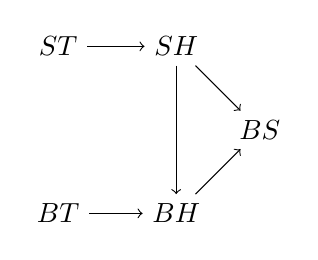
\begin{tikzpicture}[node distance={15mm}]
            \node (bs)  {$BS$};
            \node (sh) [above left of=bs] {$SH$};
            \node (bh) [below left of=bs] {$BH$};
            \node (st) [left of=sh]{$ST$};
            \node (bt) [left of=bh] {$BT$};
            \draw [->] (st) -- (sh);
            \draw [->] (sh) -- (bh);
            \draw [->] (bt) -- (bh);
            \draw [->] (sh) -- (bs);
            \draw [->] (bh) -- (bs);
        \end{tikzpicture}
    \end{figure}
    \begin{itemize}
        \item $ST$ for Suzy throws
        \item $BT$ for Billy throws
        \item $BS$ for bottle shatters
        \item $BH$ for Billy’s rock hits the (intact) bottle
        \item $SH$ for Suzy’s rock hits the bottle
        \item $BS=1$ if $SH=1$ or $BH=1$
        \item $SH=1$ if $ST=1$
        \item $BH=1$ if $BT=1$ and $SH=0$
    \end{itemize}
\end{frame}

\begin{frame}{Actual Cause}
    \begin{definition}
        $\vec X = \vec x$ is an actual cause of $\varphi$ in $(M,\vec u)$ if the following three conditions hold:
        \begin{itemize}
            \item  \textbf{AC1.} $(M,\vec u)\models (\vec X = \vec x) \wedge \varphi$.
                  (both $\vec X = \vec x$ and $\varphi$ are true in actual world)
            \item  \textbf{AC2. }There exists a partition $(\vec Z, \vec W)$ of $\mathcal{V}$ with $\vec X \subseteq \vec Z$ and some setting $(\vec x',\vec w')$ of the variables in $(\vec X,\vec W)$ such that if $(M,\vec u)\models \vec Z = z^*$ for all $Z\in \vec Z$, then both of the following conditions hold:

                  (a) $(M,\vec u)\models[\vec X \leftarrow \vec x', \vec W \leftarrow \vec w']\neg \varphi$.

                  (b) $(M,\vec u)\models[\vec X\leftarrow \vec x, \vec W' \leftarrow \vec w', \vec Z'\leftarrow \vec z^*]\varphi$ for all subsets $\vec W'$ of $\vec W$ and all subsets $Z'$ of $\vec Z$.

            \item  \textbf{AC3.} $\vec X$ is minimal; no subset of $\vec X$ satisfies conditions $AC1$ and $AC2$.
        \end{itemize}
    \end{definition}
\end{frame}

\begin{frame}{Actual Cause: Suzy and Billy}
    \begin{figure}
        \centering
        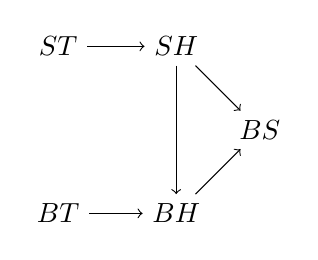
\begin{tikzpicture}[node distance={15mm}]
            \node (bs)  {$BS$};
            \node (sh) [above left of=bs] {$SH$};
            \node (bh) [below left of=bs] {$BH$};
            \node (st) [left of=sh]{$ST$};
            \node (bt) [left of=bh] {$BT$};
            \draw [->] (st) -- (sh);
            \draw [->] (sh) -- (bh);
            \draw [->] (bt) -- (bh);
            \draw [->] (sh) -- (bs);
            \draw [->] (bh) -- (bs);
        \end{tikzpicture}
    \end{figure}
    \begin{itemize}
        \item ST = 1 is a cause of BS = 1 under the contingency of BT = 0
        \item BT = 1 is not a cause of BS = 1
    \end{itemize}
\end{frame}

\begin{frame}{Extended Causal Model}
    In an extended causal model $\mathcal{E}$ specifies the set of allowable settings for the endogenous variables
    \begin{definition}
        $\vec X = \vec x$ is an actual cause of $\varphi$ in $(M,\vec u)$ if the following three conditions hold:
        \begin{itemize}
            \item  \textbf{AC1.} $(M,\vec u)\models (\vec X = \vec x) \wedge \varphi \wedge $.
            \item  \textbf{AC2. }There exists a partition $(\vec Z, \vec W)$ of $\mathcal{V}$ with $\vec X \subseteq \vec Z$ and some setting $(\vec x',\vec w')$ of the variables in $(\vec X,\vec W)$ such that if $(M,\vec u)\models \vec Z = z^*$ for all $Z\in \vec Z$, then both of the following conditions hold:
    
                  (a) $(M,\vec u)\models[\vec X \leftarrow \vec x', \vec W \leftarrow \vec w']\neg \varphi 
                  \wedge \vec V = \vec v
                  \wedge  \vec v \in \mathcal{E}$.
    
                  (b) $(M,\vec u)\models[\vec X\leftarrow \vec x, \vec W' 
                  \leftarrow \vec w', \vec Z'\leftarrow \vec z^*]
                  \vec V = \vec v \wedge (\vec v \in \mc{E} \Rightarrow \varphi)$
                      for all subsets $\vec W'$ of $\vec W$ and all subsets $Z'$ of $\vec Z$.
    
            \item  \textbf{AC3.} $\vec X$ is minimal; no subset of $\vec X$ satisfies conditions $AC1$ and $AC2$.
        \end{itemize}
    \end{definition}
\end{frame}